\section{Vegen videre for anlegget}
\thispagestyle{fancy}

Sjølv om bacheloroppgåva vår avsluttast har vi fått ein ny fascinasjon for ein sjult sektor innan offentleg infrastruktur. 
Vi ønskjer å diskutere vegen vidare for anlegget og eventuelle oppgraderingar som kan gjerast for å optimalisere prosessen.


\subsection{Ombygging}

Dersom den teoretiske bacheloroppgåva skal realiserast i praksis, treng anlegget fysiske oppgraderingar.
Reinseanlegget tilfredsstiller ikkje fleire relevante lover og forskrifter innanfor industri og offentleg infrastruktur.
Mykje av denne delen ligg utanfor vårt fokusområde, men reinseanlegget har t.d. ingen handtering eller moglegheiter for naudstopp.
Det er viktig at programmet ikkje blir sett i drift utan at anlegget går gjennom ein grundig sikkerheitsanalyse.

\begin{figure}[htbp]
    \centering
    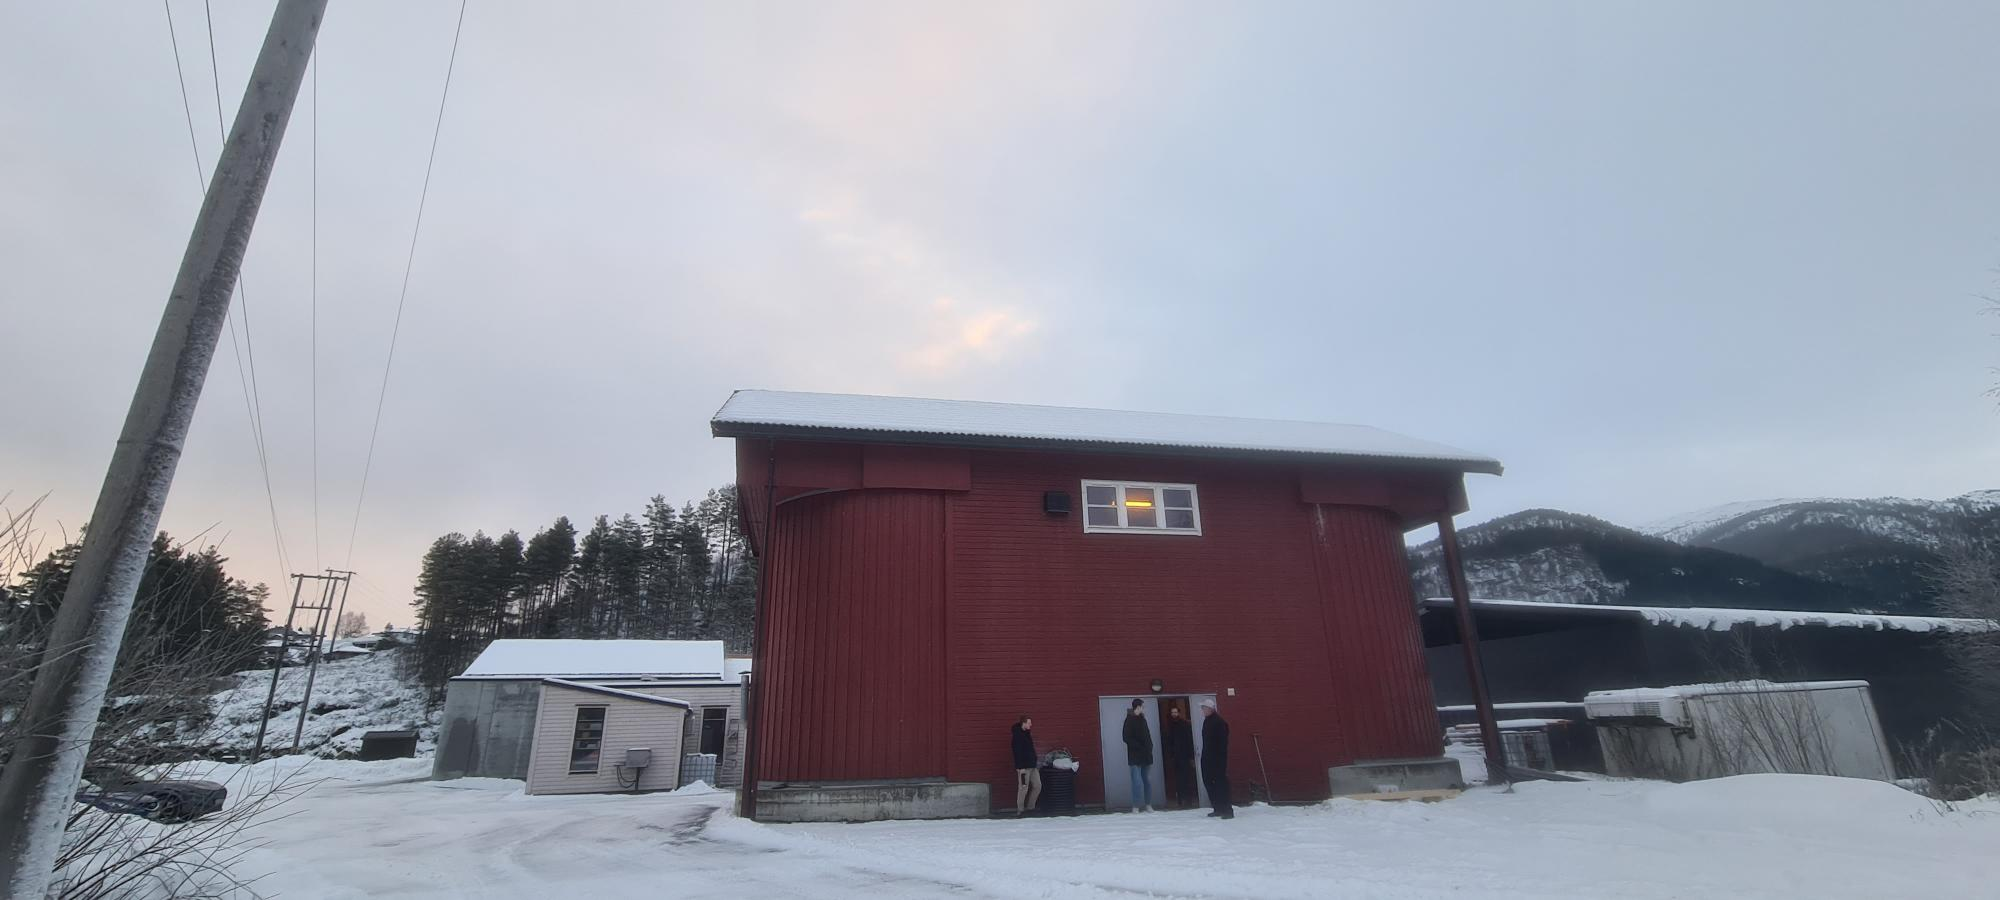
\includegraphics[width=1\textwidth]{Bilder/SandeGjennomgang.jpg}
    \caption{Første gjennomgangen av anlegget}\label{fig:Bilete Gjennomgang}
\end{figure}

\begin{center}
    \textit{Foto: Håvar Dankel}
\end{center}

\newpage

\subsection{Anbefalingar sensorikk}

For å forbetre anlegget og styresystemet ytterlegare, vil det vere nyttig å få inn meir instrumentering. 
Sensorikk vil forbetre styresystemet ved å samle meir og nøyaktig data om tilstand og ytelse. 
Med auka datamengder vil styresystemet kunne operere meir automatisk og vil kunne tilpasse seg varierande forhold meir effektivt. 
Systemet vil og ha høve til å oppdage avvik og reagere tidlegare utan manuelle inngrep, som ytterlegare aukar automasjonsevna.

Basert på vår nyerfarte kunnskap om anlegget og styresystemet, presenterer vi ei
anbefaling for oppgradering av instrumentering. 
Sjølv om all sensorikk vil være verdifull, har vi vurdert kost-nytte og anbefaler kun sensorikk som gir tilstrekkeleg verdi.


\begin{itemize}
    \item \textbf{Strøymningsmålar} \newline
        Ein strøymningsmålar vil gi nøyaktige mål på flyt av vatn.
        Dette vil forbetre kontroll på aktivering av høgbelastningsmodus, samt kontroll over og rapportering av driftsdata.
        Fleire strøymningsmålarar er moglege men minimumsanbefalinga er på vatn inn og ut av anlegget.
    \item \textbf{Energimåling} \newline
        Energimåling vil gi moglegheit for å analysere energiforbruket for å redusere kostnader og effektivisere prosessar.
        Energimåling spesifikt for komponentar kan også brukast til overvaking av utstyr for å oppdage slitasje og feil.
    \item \textbf{Reaktormålingar} \newline
        Målingar av oksygen, pH og temperatur er kritiske for å oppnå god biologisk reinsing i reaktorane \citep{SNL_PH}. \newline
        Ved å ha kontroll på desse parameterane vil reaktor kunne finjusterast for å effektivisere den biologiske reinseprosessen.
    \item \textbf{Tilbakemeldingar} \newline
        Anlegget har begrensa tilbakemeldingar frå utstyr, spesielt innan ventilstyring.
        Tilbakemeldingar er essensielt for prosesstyring, feiloppdaging og sikkerheit.
        Utan tilbakemeldingar er reinseanlegget meir sårbart for feil som ikkje blir oppdaga, 
        og slike situasjonar vil kunne resultere i nedetid, overlaup og andre utilsikta hendelser.
    \item \textbf{Forbetra nivåmåling} \newline
        Forbetring av eksisterande nivåmålingar vil gi betre mål på slammengde og slamnivå i reaktorane.
        Dette vil gjere det mogleg å nøyaktig finne skilje mellom slam og reinsa vatn etter ein sedimenteringssekvens.
    \item \textbf{Oppløysning} \newline
        Oppløysninga på analoge målingar er idag kun 0-1000 bit på 4-20mA. (Vedlegg I.12)\newline
        Oppgradering av måleoppløysning vil gjere kvar eksisterande og nye analoge målingar
        meir nøyaktig, som igjen gir moglegheit for betre styring og regulering.
\end{itemize}
\newpage


